\section{Data and Methodology}
\label{sec:data}

\subsection{Surveys:  KiDS, BOSS and 2dFLenS}
\label{sec:surveys}

The Kilo-Degree Survey \citep[KiDS,][]{dejong/etal:2013}, spans 1350 sq degrees split into two fields, one
equatorial and one southern.    Matched-depth imaging in nine bands spans the optical,
$urgi$, through to the near-infra-red, $ZYJHK_{\rm s}$, where the
near-infra-red imaging was taken as part of the KiDS partner survey
VIKING \citep[the VISTA Kilo-degree INfrared Galaxy
survey,][]{edge/etal:2013}.  High quality seeing was
routinely allocated to the primary KiDS $r$-band VST-OmegaCAM observations, resulting in a
mean $r$-band seeing of 0.7 arcseconds, with a time-allocated seeing maximum of 0.8
arcseconds.  This combination of full-area spatial and wavelength
resolution over a thousand square degrees,
provides a unique weak lensing survey that allows for enhanced
control of systematic errors \citep{giblin/etal:inprep, hildebrandt/etal:inprep}.
This analysis uses data from the fourth KiDS
data release of 1006 square degrees of imaging, (hence the name KiDS-1000), which has an effective
area, after masking, of 777 square degrees.  KiDS is a public survey from the European Southern
Observatory, with data products freely accessible through the ESO
archive\footnote{KiDS data access: \href{http://kids.strw.leidenuniv.nl/DR4}{kids.strw.leidenuniv.nl/DR4}}.   

\citet{giblin/etal:inprep} presents a series of null-tests to validate the KiDS-1000 shear catalogue in five tomographic bins spanning a 
photometric redshift range of $0.1 < z_{\rm B} < 1.2$ (see Appendix~\ref{app:properties} for details of the properties of each bin).  
Meeting their requirement that any systematic detected induces less than a $0.1\sigma$ change in the inferred 
cosmic shear constraints on the clustering cosmological parameter $S_8 = \sqrt{\sigma_8 \Omega_m/0.3}$, they conclude that the shear catalogues are `science-ready'.
\citet{hildebrandt/etal:inprep} presents a cross-correlation clustering analysis to validate the fiducial KiDS-1000 photometric redshift calibration determined using the self-organising map (SOM) methodology of \citet{wright/etal:2020}.   The SOM identifies and excludes any galaxies that are poorly represented in the spectroscopic sample, in terms of their 9-band colours and magnitudes. The resulting `gold' photometric sample, with an accurately calibrated redshift distribution, is then re-simulated in the KiDS image simulations of \citet{kannawadi/etal:2019} in order to determine the shear calibration corrections for each tomographic bin, and an associated uncertainty \citep[see][for full details]{giblin/etal:inprep,hildebrandt/etal:inprep}.
 
The Baryon Oscillation Spectroscopic Survey
\citep[BOSS,][]{alam/etal:2015}, spans an effective area of 9329 square
degrees, with spectroscopic redshifts for 1.2 million luminous red
galaxies (LRG) in the redshift range $0.2<z<0.9$.   A range of
different statistical analyses of the clustering of BOSS galaxies have been used in combination with CMB
measurements, to set tight contraints on extensions to the standard
flat $\Lambda$CDM model \citep[see][and references
therein]{alam/etal:2017}.   We adopt the anisotropic clustering
measurements of \citet{sanchez/etal:2017} in this multi-probe analysis.
BOSS only overlaps with the equatorial stripe
of the KiDS survey, with 409 square degrees of the BOSS survey lying within
the KiDS-1000 footprint.  BOSS galaxies in this overlapping region are used as lenses in
our galaxy-galaxy lensing analysis, with an effective lens number density of 0.031
galaxies per square arcmin (see Appendix~\ref{app:properties} for details).  BOSS is a public survey from the third Sloan
Digital Sky Survey\footnote{BOSS data access: \href{https://data.sdss.org/sas/dr12/boss/lss/}{data.sdss.org/sas/dr12/boss/lss/}}.   

The 2-degree Field Lensing Survey
\citep[2dFLenS,][]{blake/etal:2016}, spans 731 square degrees, with
spectroscopic redshifts for 70,000 galaxies out to $z<0.9$.   This
galaxy redshift survey from the Anglo-Australian Telescope was designed
to target areas already mapped by weak lensing surveys to facilitate `same-sky'
lensing-clustering analyses
\citep{johnson/etal:2017,amon/etal:2018,joudaki/etal:2018, blake/etal:2020}.
We use data from the 2dFLenS LRG sample that was targeted to match
the BOSS-LRG selection, but with sparser sampling.  2dFLenS
thus provides an additional sample of BOSS-like galaxies in the KiDS
southern stripe where there is 425 square degrees of overlap within
the KiDS-1000 footprint.  2dFLenS galaxies in this overlapping region are used as lenses in
our galaxy-galaxy lensing analysis, with an effective lens number density of 0.012
galaxies per square arcmin (see Appendix~\ref{app:properties} for details).  2dFLenS is a public survey\footnote{2dFLenS data
  access: \href{http://2dflens.swin.edu.au/data.html}{2dflens.swin.edu.au/data.html}}.   

\subsection{Cosmic Shear}
\label{sec:cosmic_shear}
The observed cosmic shear angular power spectrum, $C_{\epsilon \epsilon}(\ell)$, measures a combination of the distortions arising from weak gravitational lensing by large scale structures (labelled with a subscript `G') with a low-level contaminating astrophysical signal arising from the intrinsic alignment of galaxies with the large scale structures within which they are embedded (labelled with a subscript `I').   These contributions can be separated as
\be
\label{eq:cl_cosmicshear}
C^{(ij)}_{\epsilon \epsilon}(\ell) = C^{(ij)}_{\rm GG}(\ell) +
C^{(ij)}_{\rm GI}(\ell) + C^{(ij)}_{\rm IG}(\ell) + C^{(ij)}_{\rm II}(\ell)\;,
\ee
where the indices $i$ and $j$ indicate cross-correlations between the five tomographic source samples.   The theoretical power spectra are given by Limber-approximated projections with
\be
\label{eq:generallimber}
C^{(ij)}_{\rm ab}(\ell) = \int^{\chi_{\rm hor}}_0 \!\!\! \dd \chi\;
\frac{W^{(i)}_{\rm a} (\chi)\; W^{(j)}_{\rm b} (\chi)}{f^2_{\rm
    K}(\chi)}\; P_{\rm m, nl} \br{\frac{\ell+1/2}{f_{\rm K}(\chi)},z(\chi)}\;,
\ee
where ${\rm a,b} \in \bc{\rm I,G}$, $f_{\rm K}(\chi)$ is the comoving angular diameter distance and $\chi$ is the comoving radial distance which runs out to the horizon, $\chi_{\rm hor}$.  The weight functions, $W(\chi)$, encode information about the KiDS-1000 survey depth \citep[see equations 15 and 16 of][]{joachimi/etal:inprep}.   In the cases of power spectra that include intrinsic `I' terms, the weight function also encodes the intrinsic galaxy alignment model which we take to be the `NLA' model from \citet{bridle/king:2007}.   The cosmological information for this statistic is contained in both the geometric weight functions, $W(\chi)$, and in the evolution and shape of the non-linear matter power spectrum, $P_{\rm m, nl}(k,z)$, which we model using the halo formalism\footnote{We calculate the non-linear power spectrum using {\sc HMCode} \citep{mead/etal:2015}, which is incorporated in {\sc CAMB} \citep{lewis/bridle:2002}.   \citet{joachimi/etal:inprep} demonstrate that the \citet{mead/etal:2015} halo model prescription provides a sufficiently accurate model of the non-linear matter power spectrum into the highly non-linear regime through a comparison to weak lensing observables emulated using the N-body CosmicEmu simulations \citep{heitmann/etal:2014}.   It also has the added benefit of allowing us to marginalise over our uncertainty on the impact of baryon feedback on the shape of the non-linear total matter power spectrum \citep{semboloni/etal:2011,mead/etal:2015,mead/etal:2020}.} of \citet{mead/etal:2015}.   Weak lensing is therefore fairly unique as a cosmological probe, as it is sensitive to changes in both the distance-redshift relation and in the growth of structures.

We estimate the cosmic shear angular power spectrum through a linear transformation of the real-space two-point shear correlation function \citep{schneider/etal:2002}.  This approach circumvents the challenge of accurately determining the survey mask for a direct power spectrum estimate.  \citet{joachimi/etal:inprep} detail the apodisation advances that we have adopted for the transformation, in addition to the modelling that we use to account for the minor differences between the theoretical expectation of the true angular power spectrum in Eq.~(\ref{eq:cl_cosmicshear}) and the measured `band powers'.    
 
Fig.~\ref{fig:Pkk} presents the \citet{asgari/etal:inprep} KiDS-1000 cosmic shear power spectra for the auto and cross-correlated tomographic bins.   Here we have constructed both E-mode (upper left) and B-mode (lower right) band powers in order to isolate any non-lensing B-mode distortions.     As expected from the analysis of \citet{giblin/etal:inprep}, the measured B-modes are found to be consistent with zero.   The measured E-modes can be compared to the theoretical expectation given the best-fit set of cosmological parameters from our joint multi-probe analysis in Sect.~\ref{sec:results}.



\begin{figure*}
        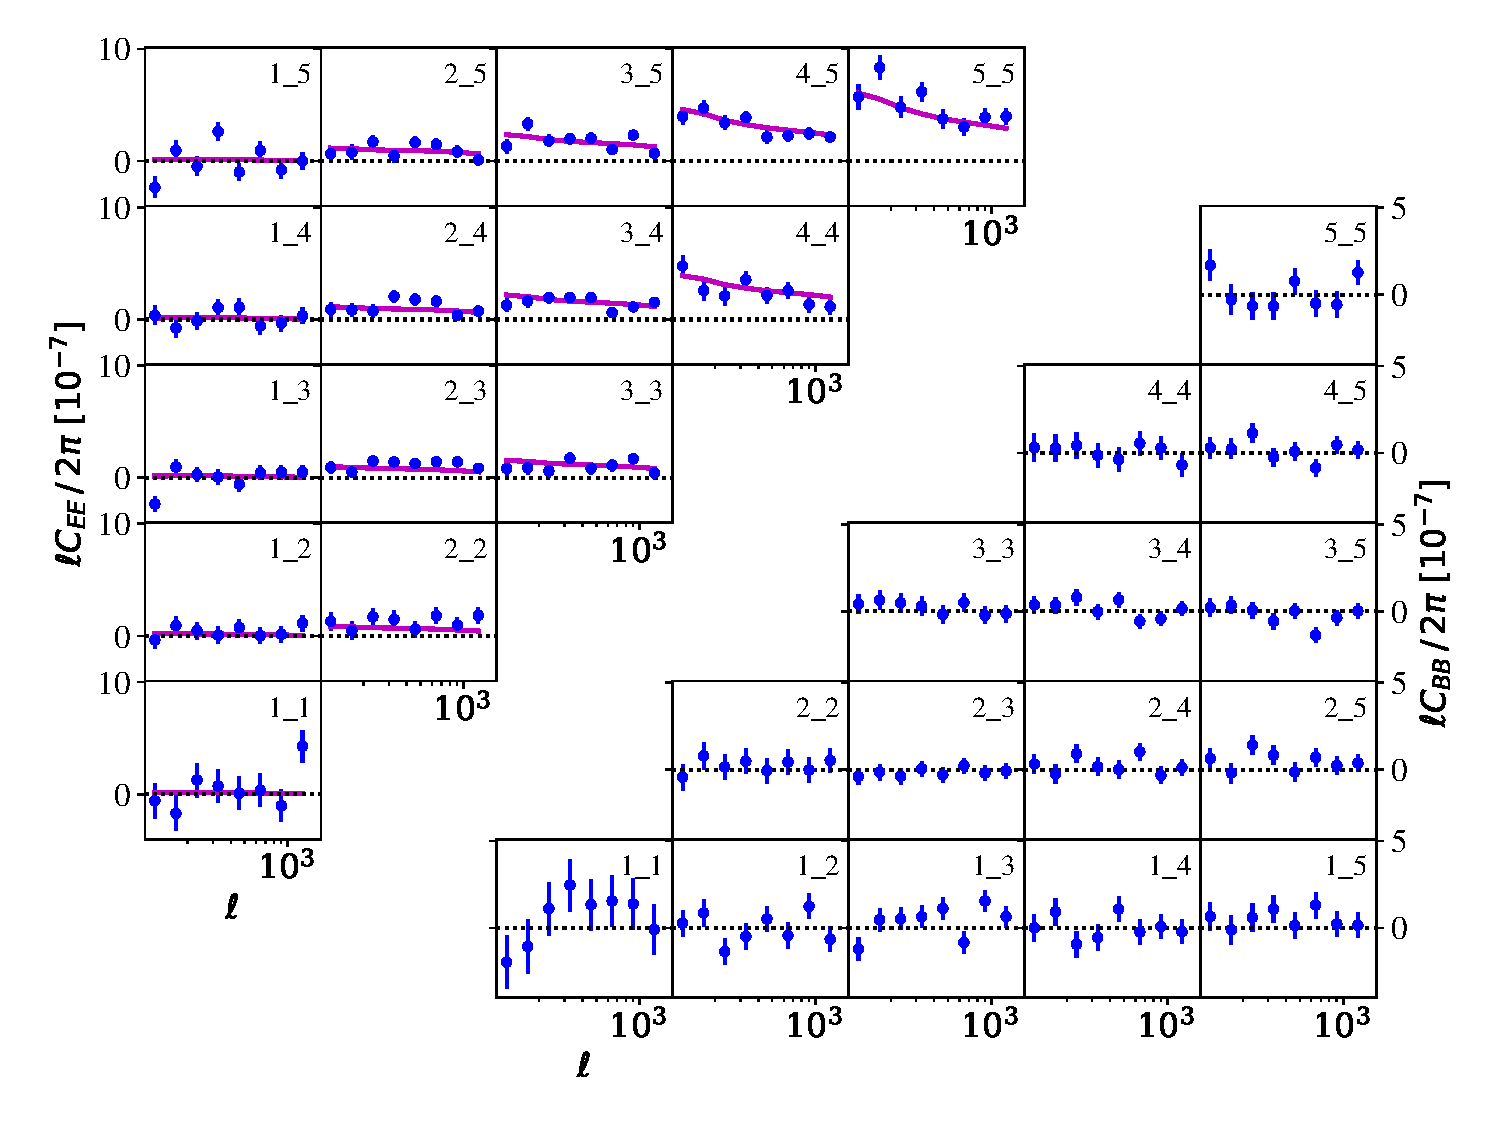
\includegraphics[width=\textwidth]{Data_Plots/Pkk/Pkk_K1000_2Dbins_v2_goldclasses_Flag_SOM_Fid_A.pdf}
        \caption{KiDS-1000 cosmic shear power spectra:  Tomographic
          band powers comparing the E-modes (upper left block) with the best-fit
          cosmological model from our combined multi-probe analysis.  The tomographic
        bin combination is indicated in the upper right corner of each
      sub-panel.  The null-test B-modes (lower right block), are
      consistent with zero for both the full data vector, and each
     bin combination individually.}
        \label{fig:Pkk}
\end{figure*}


\subsection{Anisotropic Galaxy Clustering}
\label{sec:clustering}
Galaxy clustering observations probe the 3D non-linear galaxy-galaxy power spectrum and we follow \citet{sanchez/etal:2017} in modelling this quantity based on a perturbation theory approach with
\be
\label{eq:pgg}
P_{\rm gg}(k,z) = \sum_{\alpha,\beta} \alpha\, \beta\, P_{\alpha
  \beta}(k,z) + b_1 \gamma_3^-\, P_{b_1 \gamma_3^-}(k,z) + P_{\rm noise}(k,z)\;.
\ee
Here $\alpha,\beta \in \bb{b_1, b_2, \gamma_2}$, introducing the linear and quadratic bias parameters $b_1$ and $b_2$, in addition to the non-local bias parameters $ \gamma_2$ and $\gamma_3^-$.  Each of the power spectrum terms on the right hand side of the equation are given by different convolutions of the linear matter power spectrum in appendix A of \citet{sanchez/etal:2017}.   In the case of an effective linear galaxy bias model \citep[see for example][]{vanuitert/etal:2018, abbott/etal:2018} only the $b_1$ bias parameter is considered to be non-zero and Eq.~(\ref{eq:pgg}) reduces to $P_{\rm gg}(k,z) =b_1^2 P_{\rm m, nl}^{\rm pert}(k,z)$, where $P_{\rm m, nl}^{\rm pert}(k,z)$ is the pertubation theory estimate of the non-linear matter power spectrum which is accurate at the percent level to $k \lesssim 0.3 h \,{\rm Mpc}^{-1}$.

\citet{sanchez/etal:2017} present the anisotropic redshift-space correlation function of galaxy clustering, with the galaxy pairs separated into three `wedges' equidistant in $\mu$, where $\mu$ is the cosine of the angle between the line of sight and the line connecting the galaxy pairs.   As such the 3D correlation function is measured for pairs that are either mainly transverse to the line of sight, mainly parallel to the line of sight, or placed into an intermediate sample between these two cases.  The redshift-space correlation functions $\xi_{\rm gg} \br{s,\mu,z}$, where $s$ is the co-moving galaxy-pair separation, is given by
\eqa{
\label{eq:bosswedgefouriertrafo}
 \xi_{\rm gg} \br{s,\mu,z} &= \sum_{l=0}^{2} L_{2l}(\mu) \frac{(-1)^l
   (4l+1)}{(2 \pi)^2} \int_0^\infty \dd k\, k^2 {\rm j}_{2l}(ks) \\ \nonumber
& \times \int_{-1}^1
 \dd \mu_1 L_{2l}(\mu_1) P_{\rm gg, s}(k,\mu_1,z)\;,
}
where $L_i$ denotes the Legendre polynomial of degree $i$, ${\rm j}_i$ is the spherical Bessel function of order $i$ and $P_{\rm gg, s}(k,\mu_1,z)$ is the 3D redshift-space power spectrum that includes the non-linear real-space power spectrum, Eq.~(\ref{eq:pgg}), and the galaxy-velocity and velocity-velocity power spectrum \citep[see][for details]{sanchez/etal:2017}.   

Fig.~\ref{fig:wedges} presents the \citet{sanchez/etal:2017} BOSS-DR12 anisotropic clustering correlation functions in three wedges.   The measured correlation functions can be compared to the theoretical expectation given the best-fit set of cosmological parameters from our joint multi-probe analysis in Sect.~\ref{sec:results}.

\begin{figure*}
        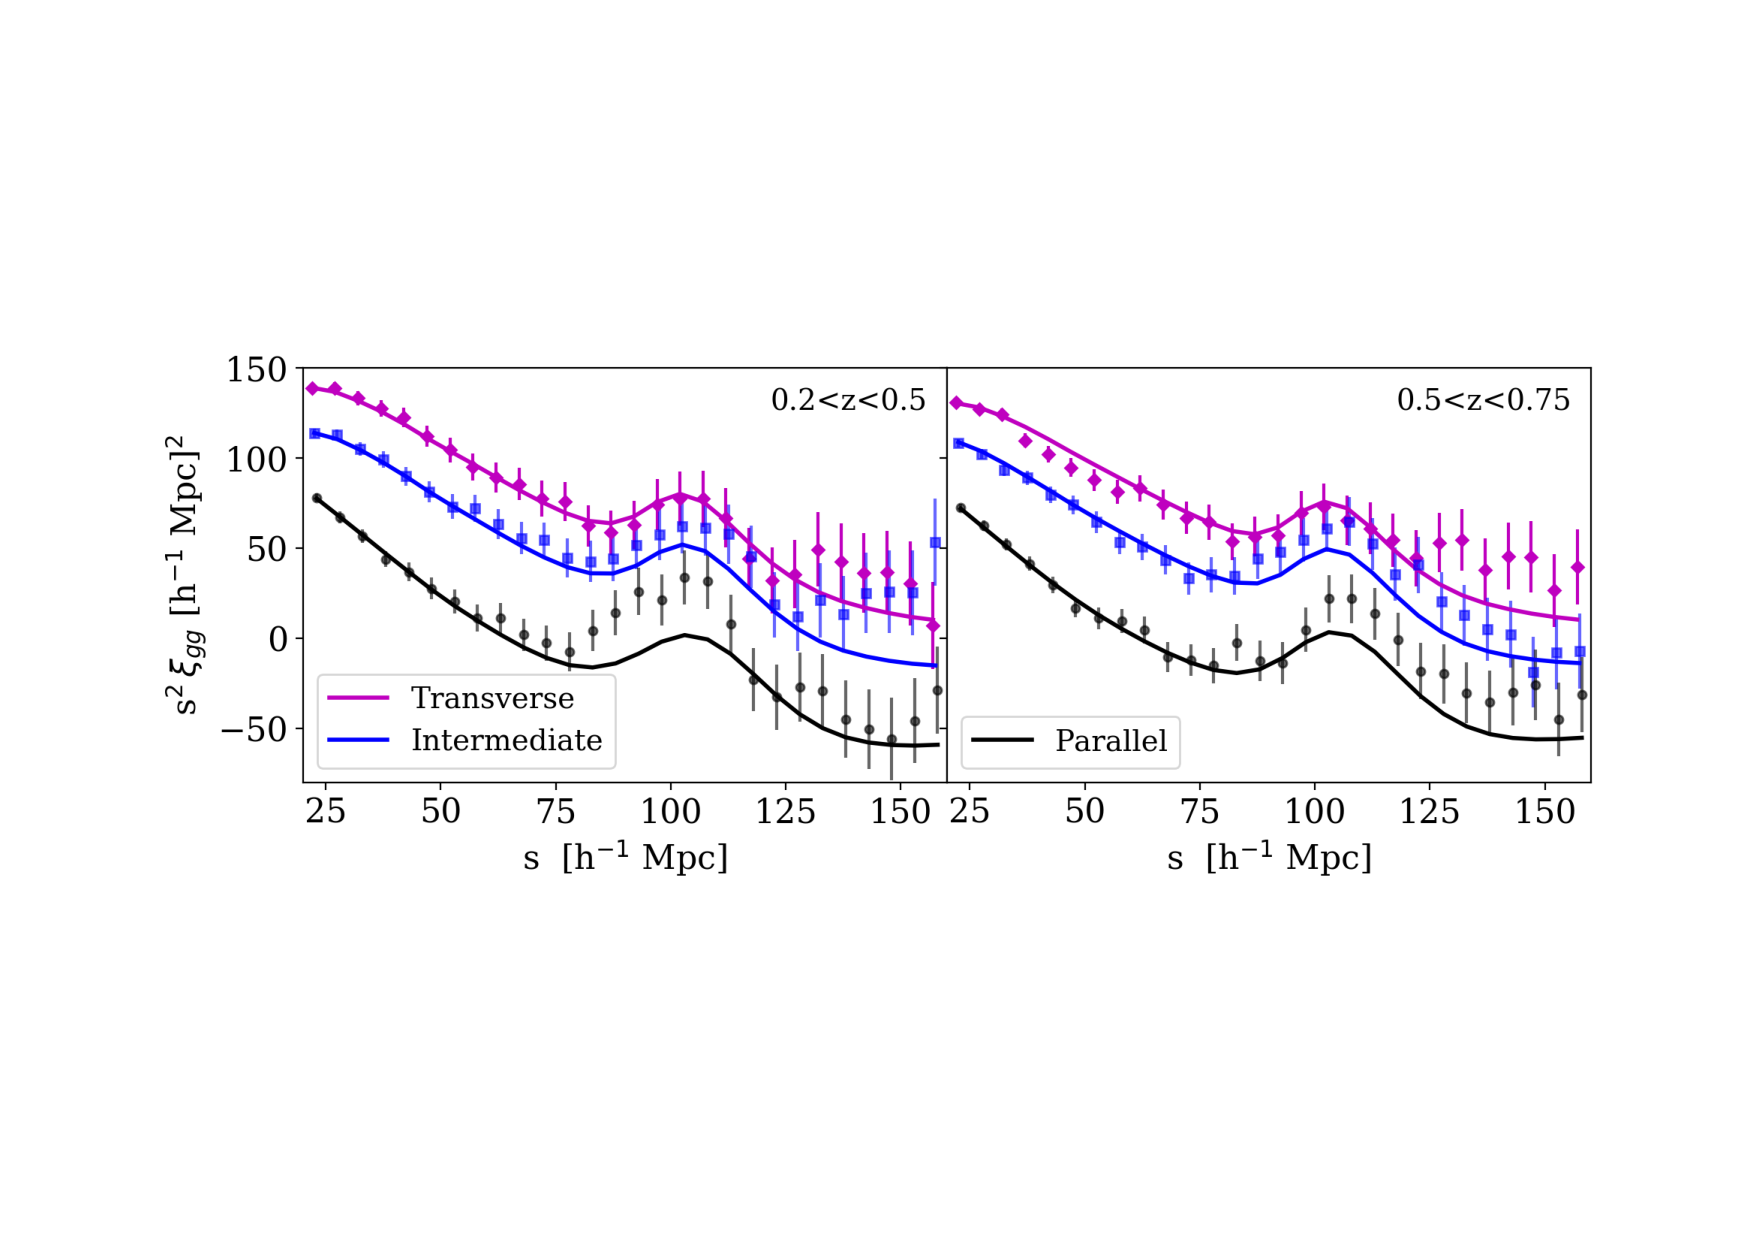
\includegraphics[width=\textwidth]{Data_Plots/clustering_wedges/BOSS_Sanchez_wedges.pdf}
        \caption{BOSS-DR12 anisotropic clustering from \citet{sanchez/etal:2017}:
          The transverse (pink), intermediate (blue) and parrallel
          (black) clustering wedges in two redshift bins, compared 
          with the best-fit
          cosmological model from our combined multi-probe analysis.}
        \label{fig:wedges}
\end{figure*}

\subsection{Galaxy-Galaxy Lensing}
\label{sec:GGL}
The observed galaxy-galaxy lensing angular power spectra, $C_{\rm n \epsilon}(\ell)$, measures a combination of weak lensing distortions around foreground galaxies (labelled with a subscript `gG') with a low-level intrinsic alignment signal arising from the fraction of the source galaxy population that reside physically close to the lenses (labelled with a subscript `gI').   We also consider the low-level lensing-induced magnification bias (labelled with a subscript `mG').   These three contributions can be separated as 
\be
\label{eq:cl_ggl}
C^{(ij)}_{\rm n \epsilon}(\ell) = C^{(ij)}_{\rm gG}(\ell) +
C^{(ij)}_{\rm gI}(\ell) + C^{(ij)}_{\rm mG}(\ell)  \;,
\ee
where the index $i$ indicates the two lens galaxy samples, and the index $j$ indicates the five tomographic source samples.   The theoretical power spectra are given by Limber-approximated projections following Eq.~(\ref{eq:generallimber}), with two key differences.   The first is that the lens weight function is replaced by the redshift distribution of the lenses.   The second is that the non-linear matter power spectrum is replaced with the non-linear cross power spectrum between the galaxy and matter distribution $P_{\rm gm}(k,z)$ \citep[see equations 24 and 25 of][for the full expressions]{joachimi/etal:inprep}.   For the magnification bias power spectrum, $C_{\rm mG}(\ell)$, we refer the reader to appendix B in \citet{joachimi/etal:inprep}.   We find that the inclusion or exclusion of this term has a negligible impact on our cosmological constraints, but we retain it nevertheless.

We adopt the non-linear galaxy bias model from \citet{sanchez/etal:2017}, and approximate the non-linear cross power spectrum as
\eqa{
\label{eq:pgm}
P_{\rm gm}(k,z) &= b_1 P_{\rm m, nl}(k,z) + \left\{ b_2\, {\cal F}_{b_2}(k)
  - \gamma_2\, {\cal F}_{\gamma_2}(k) \right.\\ \nonumber
& \left. -\, \gamma_3^-\, {\cal F}_{\gamma_3^-}(k)
 \right\} P_{\rm m, lin}^{2}(k,z)\;,
}
where the logarithm of the functions ${\cal F}_\alpha(k)$ are second-order polynomial fits that we use to model $P_\alpha(k,z_{\rm ref})/P^2_{\rm m, lin}(k,z_{\rm ref})$, the ratio between the different bias terms in the full pertubation theory model in Eq.~(\ref{eq:pgg}), and the square of the linear matter power spectrum.  This approach permits a reasonable extrapolation of the \citet{sanchez/etal:2017} pertubation model into the non-linear regime beyond $k = 0.3 h \,{\rm Mpc}^{-1}$.   This is necessary in order to carry out the redshift-weighted projection of the 3D model to estimate the 2D galaxy-galaxy lensing observable (Eq.~\ref{eq:generallimber}).  No matter which $\ell$-scales we restrict our analysis to, high $k$-scales will contribute to all scales at some degree \citep{joachimi/etal:inprep, asgari/etal:2020}.   This approach also yields a several order of magnitude speed-up over the direct perturbative calculations, significantly reducing the galaxy-galaxy lensing likelihood evaluations.  

Fig.~\ref{fig:Pgk} presents the KiDS-1000 galaxy-galaxy lensing power spectra, around lenses from the BOSS and 2dFLenS surveys \citep[see][for the real-space KiDS-1000 galaxy-galaxy lensing measurements for BOSS and 2dFLenS separately]{blake/etal:2020}.   Each panel presents the cross correlation between each of the five different tomographic source bins, denoted `S', with the two different lens bins, denoted `L' (see Table~\ref{tab:datatab} for details).  Here we have constructed both E-mode (left) and B-mode (right) band powers in order to isolate any non-lensing B-mode distortions.     As expected from the analysis of \citet{giblin/etal:inprep}, the measured B-modes are found to be consistent with zero.   The measured E-modes can be compared to the theoretical expectation given the best-fit set of cosmological parameters from our joint multi-probe analysis in Sect.~\ref{sec:results} in the non-shaded regions.    

The shaded regions in Fig.~\ref{fig:Pgk} are excluded from our analysis for two reasons.   For overlapping lens-source bins (L1 with S1 and L2 with S1 to S3), the intrinsic alignment terms $C_{\rm gI}(\ell)$ are expected to become significant.   This raises the question of the validity of the arguably rudimentary `NLA' intrinsic alignment model when used in combination with a non-linear galaxy bias model \citep[see][for a self-consistent pertubative approach to both intrinsic alignment and galaxy bias modelling]{blazek/etal:2019}.   As these bins carry little cosmological information, we exclude this data from our cosmological inference analysis, using it instead in a redshift-scaling null test of the catalogue in \citet{giblin/etal:inprep}.   For separated lens-source bins we introduce a maximum $\ell$-scale beyond which the contributions from scales $k > 0.3 h \,{\rm Mpc}^{-1}$ become significant \citep[see figure 2 in][]{joachimi/etal:inprep}  In this regime uncertainties in the extrapolation of the \citet{sanchez/etal:2017} non-linear galaxy bias model into the non-linear regime (Eq.~\ref{eq:pgm}) renders the $C_{\rm n \epsilon}(\ell)$ model invalid.   The $\ell$-limit depends on the redshift of the lens bin.    Fig.~\ref{fig:Pgk} therefore serves as important illustration of the necessity of improving non-linear galaxy bias modelling for future studies, in order to fully exploit the cosmological signal contained within the galaxy-galaxy lensing observable.


\begin{figure*}
        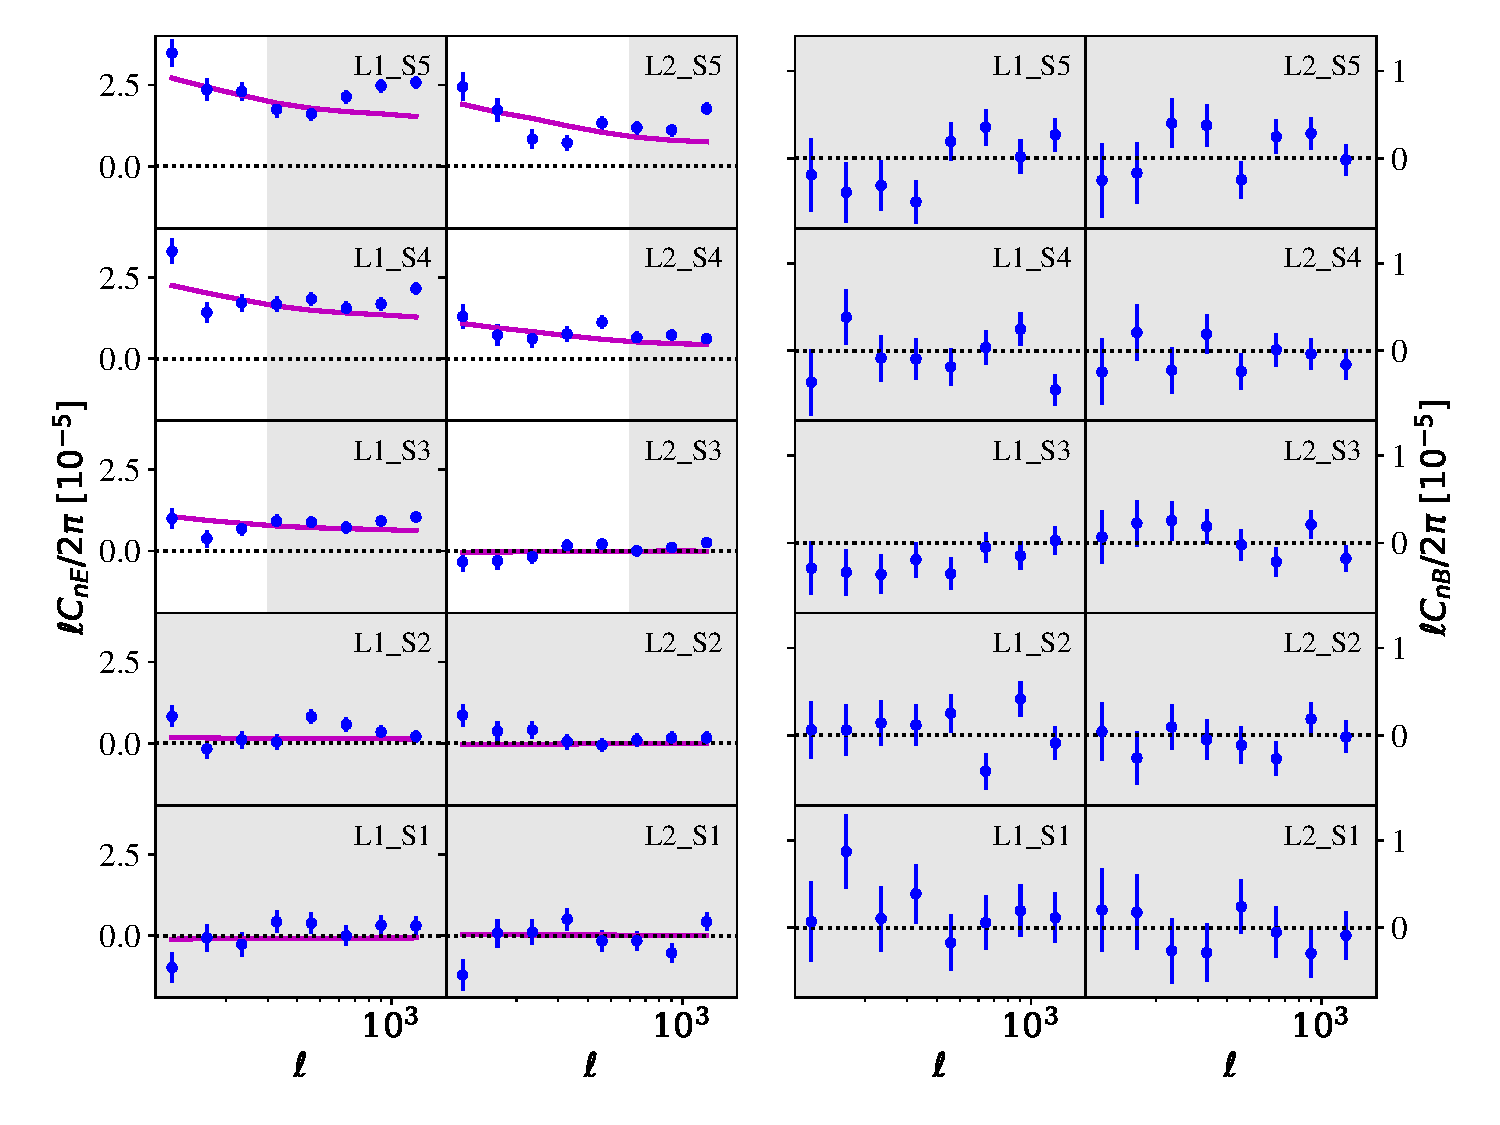
\includegraphics[width=\textwidth]{Data_Plots/Pgk/Pgk_K1000_2Dbins_v2_goldclasses_Flag_SOM_Fid_A.pdf}
        \caption{KiDS-1000 galaxy-galaxy lensing power spectra:
          Tomographic band powers comparing the E-modes (left block)
          with the best-fit
          cosmological model from our combined multi-probe analysis.  The tomographic 
        bin combination of BOSS and 2dFLenS lenses (L) with KiDS-1000
        sources (S), is indicated in the upper right corner of each
        sub-panel.  Data within grey-regions are not included in the cosmological analysis.
        The null-test B-modes (right block), are
      consistent with zero for both the full data vector, and each
     bin combination individually.}
        \label{fig:Pgk}
\end{figure*}



\subsection{Multi-Probe Covariance}
\label{sec:Cov}
\citet{joachimi/etal:inprep} present the multi-probe covariance matrix adopted in this study, verified through an analysis of over 20,000 fast full-sky mock galaxy catalogues derived from lognormal random fields.   Given that only 4\% of the BOSS footprint overlaps with KiDS-1000, in an initial step we validate the approximation that the BOSS anisotropic galaxy clustering observations are uncorrelated with the cosmic shear and galaxy-galaxy lensing observations.   By imposing realistic overlapping BOSS and KiDS-1000 footprints in our mock catalogues, we find that cross-correlation, between the projected BOSS-like angular galaxy correlation function, and the KiDS-1000-like weak lensing signals, is less than $\sim 5\%$ of the auto-correlation terms along the diagonal of covariance matrix.  With such a low cross-correlation, we can safely assume independence between the clustering and lensing observations, allowing us to adopt the \citet{sanchez/etal:2017} covariance matrix\footnote{The BOSS $\xi_{\rm gg}$ covariance is derived from the {\sc MD-Patchy} BOSS mock catalogues of \citet{kitaura/etal:2016}.} for the anisotropic galaxy clustering observations, $\xi_{\rm gg}(s,\mu,z)$, setting the clustering-lensing cross-correlation terms to zero.   

The covariance of the two weak lensing observations is calculated analytically, combining terms that model pure Gaussian shape noise, survey sampling variance and the noise-mixing that occurs between these two components, in addition to higher-order terms that account for mode-mixing between the in-survey modes and between the observed in-survey and the unobserved out-of-survey modes \citep[known as super-sample covariance,][]{takada/hu:2013}.   The covariance also includes a contribution to account for our uncertainty on the multiplicative shear calibration correction \citep{kannawadi/etal:2019}.  \citet{joachimi/etal:inprep} demonstrate that every term in the covariance is important to model, with each term found to dominate in different regions of the covariance.   It is therefore important to review the approximations made in these analytical calculations.    Whilst the complex KiDS-1000 footprint is fully accounted for in the shape-noise terms, and the super-sample terms,  the survey is approximated as a contiguous square footprint, the size of the effective survey area for all other terms.   Furthermore, the survey is assumed to be homogenous in its depth, which is invalid for any ground-based survey where the survey depth becomes a sensitive function of the observing conditions \citep{heydenreich/etal:2020}.   With mock catalogues, we have the freedom to impose complex masks and variable depth to quantify the impact of these effects on the derived covariance, finding differences typically $\lesssim 10\%$, with a maximum difference of $\sim 20 \%$.  The majority of the differences were found to be driven by the mix-term between the Gaussian shape noise and the Gaussian sampling variance.    Through a mock multi-probe data vector MCMC analysis, \citet{joachimi/etal:inprep} demonstrate that these differences in the covariance are not expected to lead to any systematic bias in the recovery of the KiDS-1000 cosmological parameters, nor to any significant differences in the confidence regions of the recovered parameters.   We therefore adopt an analytical covariance in our analysis,  and refer the reader to \citet{joachimi/etal:inprep} for further details, where their section 4 presents the mocks, section 5 and appendix E presents the analytical covariance model and appendix D presents detailed comparisons of the mock and analytical covariance.

\subsection{Parameter Inference methodology}
\label{sec:KCAP}
We use the KiDS Cosmology Analysis Pipeline, {\sc KCAP}\footnote{KCAP will be made public on acceptance of the KiDS-1000 analysis papers.   Interested groups can however request early access by e-mail to the lead authors of this paper.} built from the {\sc CosmoSIS} analysis framework of \citet{zuntz/etal:2015}, adopting the nested sampling algorithm {\sc Multinest} \citep{feroz/hobson:2008,feroz/etal:2009,feroz/etal:2019}.  The {\sc KCAP} bespoke modules include the BOSS wedges likelihood from \citet{sanchez/etal:2017}, the galaxy-galaxy lensing likelihood based on Eq.~(\ref{eq:pgm}), and tools to permit correlated priors on nuisance parameters and accurate sampling over the clustering parameter $S_8= \sigma_8 \sqrt{\Omega_{\rm m}/0.3}$, a parameter which is typically only derived.  Scripts are also provided to derive the best-fit parameter values at the maximum multivariate posterior, denoted MAP (maximum a posteriori), and an associated credible region given by the projected joint highest posterior density region, denoted PJ-HPD.  This list of new modules reflect the primary updates in the KiDS-1000 parameter inference methodology compared to previous KiDS analyses.

The priors adopted in parameter inference are usually survey-specific, and are given, for this analysis, in Appendix~\ref{app:priors}.  Whilst they are intended to be uninformative on $S_8$, the parameter that lensing studies are most sensitive to, different prior choices, particularly on the amplitude of the primordial power spectrum of scale density fluctuations $A_{\rm s}$, have been shown to lead to non-negligible changes in the derived $S_8$ parameter \citep{chang/etal:2019, joudaki/etal:2020, asgari/etal:2020_KD}.   \citet{joachimi/etal:inprep} show that even with wide priors on $A_{\rm s}$,  the sampling region in the $\sigma_8 - \Omega_{\rm m}$ plane is significantly truncated at low values of $\sigma_8$ and $\Omega_{\rm m}$, with the potential to introduce a subtle bias towards low values of $\sigma_8$.   In this analysis, we negate this important issue of implicit informative priors by sampling directly in $S_8$, adopting a wide uninformative uniform prior.  We note, however, that this approach is expected to lead to a more conservative constraint on $S_8$, compared to an analysis that adopts a uniform prior\footnote{For quantitative information about the impact of implicit $A_{\rm s}$ priors, see table 5 and figure 22 of \citet{joachimi/etal:inprep}.} on $\ln A_{\rm s}$.

We account for our uncertainty in our source redshift distributions using nuisance parameters $\delta_z^i$ which modify the mean redshift of each tomographic bin $i$.   By analysing mock KiDS catalogues, \citet{wright/etal:2020} determined the mean bias per redshift bin $\mu^i$, and also the covariance between the different redshift bins, $C_{\delta z}$.   This covariance arises from sampling variance in the spectroscopic training sample, which impacts, to some degree, the redshift calibration of all bins.    We therefore adopt the multivariate Gaussian prior ${\cal N}(\vek{\mu};\vek{C}_{\delta z})$, for the vector $\vek{\delta}_z$. 

A standard approach to parameter inference reports the mean, or maximum, of the one-dimensional marginal distribution, along with a tail credible interval that encompasses 68\% of the marginal highest posterior density, denoted M-HPD.  For the high-dimensional parameter space of a multi-probe weak lensing analysis, marginalised point estimates of $S_8$ are found to be lower than the true parameter value in mock data analyses \citep{joachimi/etal:inprep}.   This is not a result of an error in the {\sc KCAP} inference pipeline.  Rather, it is a feature of the shape of the multivariate posterior distribution which exhibits multiple linear degeneracies (for example $\sigma_8$ with $\Omega_{\rm m}$ and the galaxy bias parameter $b_1$).   We note that the presence of offsets in the weak lensing marginalised $S_8$ constraints raises a flag at any efforts to accurately quantify tension between probes based solely on these one-point estimates.  Tension can only be fully assessed in terms of the overlap between the full posterior distributions \citep[see for example][]{handley/lemos:2019,lemos/etal:2019}, but as we discuss in Sect.~\ref{sec:planck_comp}, it remains a challenge to determine an accurate and meaningful quantification of tension in this way.

Adopting the Bayesian paradigm for inference, we provide our constraints in the form of a series of samples that describe the full posterior distribution\footnote{Full MCMC chains will be publicly released on the acceptance of this paper.} .    In Sect.~\ref{sec:results} we explore this multi-dimensional posterior in the traditional way, visualising the 2D and 1D marginal posterior distributions for a selection of parameters.  In order to present headline $S_8$ constraints, however, we present the parameter value at the maximum posterior (MAP), along with a credible interval based on the joint, multi-dimensional highest posterior density region, projected onto the marginal posterior of the $S_8$ parameter \citep[see section 6.4 of][for further details on this MAP with PJ-HPD estimator]{joachimi/etal:inprep}.  We note that the MAP reported by {\sc Multinest} provides a noisy estimate of the true MAP, and we therefore conduct a series of \ch{X00} \citet{nelder/mead:1965} maximum likelihood analyses, with different starting points based on the {\sc Multinest} posterior.   The reported MAP then given by the maximum likelihood point with the lowest $\chi^2$ value \citep[see also][who adopt a similar approach]{muir/etal:2020}.



 







